\section{Introduction}\label{sec:intro}

% Need a paragrapgh or two to explain why the tool is interesting and
% significant should be provided.

\dReach{} is a bounded reachability analysis tool for hybrid systems.
It encodes bounded reachability problems of hybrid systems as
first-order formulas over the real numbers, and solves them using
$\delta$-decision procedures in the SMT solver
\dReal{}~\cite{DBLP:conf/cade/GaoKC13}. \dReach{} is able to handle a
wide range of highly nonlinear hybrid systems~\cite{CMSB14,DBLP:conf/fmcad/GaoKC13,DBLP:conf/hybrid/KapinskiDSA14,6868816}.
Figure~\ref{fig:prostate-example} highlights some of its features: on
the left is an example of some nonlinear dynamics that \dReach{} can
handle, and on the right a visualized counterexample generated by
\dReach{} on this model.
\begin{figure}[!h]
  \subfloat[An example of nonlinear hybrid system model: off-treatment
  mode of the prostate cancer treatment model~\cite{CMSB14}\label{subfig-1:prostate}]{
    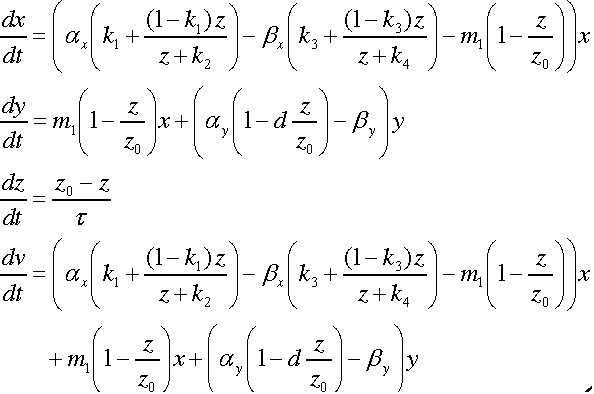
\includegraphics[width=0.45\textwidth]{images/prostatebw-mode2.pdf}
  }
  \hfill
  \subfloat[Visualization of a generated counterexample. Change in the shade of colors represents discrete mode changes.]{%
    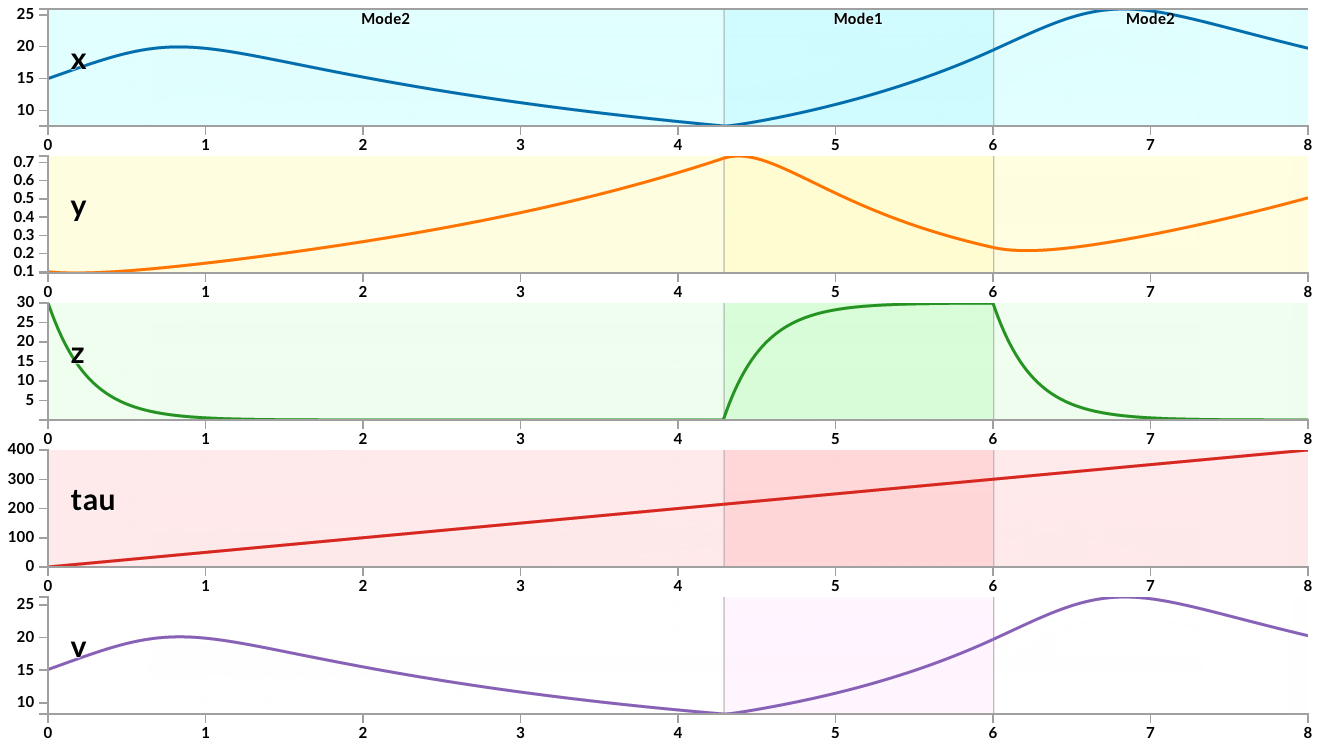
\includegraphics[width=0.48\textwidth]{images/prostate}
  }
  \caption{An example of nonlinear dynamics and counterexample-generation.}
  \label{fig:prostate-example}
\end{figure}

It is well-known that the standard bounded reachability problems for
simple hybrid systems are already highly
undecidable~\cite{DBLP:conf/hybrid/AlurCHH92}.
Instead, we work in the framework of $\delta$-reachability of hybrid systems~\cite{DBLP:journals/corr/GaoKCC14}.
Here $\delta$ is an arbitrary positive rational number, provided by the user to
specify the bound on numerical errors that can be tolerated in the analysis.
For a hybrid system $H$ and an unsafe region $\unsafe$ (both encoded as logic formulas),
the $\delta$-reachability problem asks for one of the following answers:
\begin{itemize}
        \item {\sf safe}: $H$ cannot reach $\unsafe$.
        \item {\sf $\delta$-unsafe}: $H^{\delta}$ can reach $\unsafe^{\delta}$.
\end{itemize}
Here, $H^{\delta}$ and $\unsafe^{\delta}$ encode ($\delta$-bounded) overapproximations
of $H$ and $\unsafe$, defined explicitly as their syntactic variants. (See Section~\ref{sec:delta-reachability} in the Appendix.)
It is important to note that the definition makes the answers no weaker than standard reachability:
When {\sf safe} is the answer, we know for certain that $H$ does not reach
the unsafe region (no $\delta$ is involved); when {\sf $\delta$-unsafe} is the answer,
we know that there exists some $\delta$-bounded perturbation of the system that can render it unsafe.
Since $\delta$ can be chosen to be very small, {\sf$\delta$-unsafe} answers in fact
discover robustness problem in the system, which should be regarded as unsafe indeed.
We have proved that bounded $\delta$-reachabilty is decidable for a wide range
of nonlinear hybrid systems, even with reasonable complexity bounds~\cite{DBLP:journals/corr/GaoKCC14}.
This framework provides the formal correctness guarantees of \dReach{}.

Apart from solving $\delta$-reachability, the following key features of \dReach{}
distinguish it from other existing tools in this domain~\cite{DBLP:journals/jlp/FranzleTE10,DBLP:conf/cav/FrehseGDCRLRGDM11,DBLP:journals/tac/AlthoffK14,DBLP:conf/hybrid/Frehse05,DBLP:conf/icons/HerdeEFT08,DBLP:conf/rtss/ChenAS12}.
%insert explanations for each item.

1. Expressiveness. \dReach{} allows the user to describe hybrid systems using first-order
logic formulas over real numbers with a wide range of nonlinear functions. This allows
the user to specify the continuous flows using highly nonlinear differential equations,
and the jump and reset conditions with complex Boolean combinations of nonlinear constraints.
\dReach{} also faithfully translates mode invariants into $\exists\forall$ logic formulas,
which can be directly solved under certain restrictions on the invariants.

2. Property-guided search. \dReach{} maintains logical encodings, whose size is linear in the size of the inputs, of the reachable states of
a hybrid system. The tool searches for concrete counterexamples to falsify the reachability properties, instead of overapproximating the full reachable states.
This avoids the usual state explosion problem in reachable set computation, because the full set of states does not need to be explicitly stored. This change
is analogous to the difference between SAT-based model checking and BDD-based symbolic model checking.

3. Tight integration of symbolic reasoning and numerical solving. \dReach{} delegates the
reasoning on discrete mode changes to SAT solvers, and uses numerical constraint solving to handle nonlinear dynamics.
As a result, it can combine the full power of both symbolic reasoning and numerical analysis algorithms. In particular,
all existing tools for reachable set computation can be easily plugged-in as engines for solving
the continuous part of the dynamics, while logic reasoning tools can overcome the difficulty
in handling complex mode transitions.

The paper is structured as follows. We describe the system architecture in Section 2,
and give some details about the logical encoding in the tool in Section 3.
We then explain the input format and usage in Section 4. More details and examples are given in the Appendix.

%Realistic hybrid systems involves nonlinear ODEs with transcendental
%functions. \dReach{} allows users to specify a hybrid system in a
%nonlinear signature as it is without linearizing or overapproximating
%it. Users can provide the tool with a numerical error bound $\delta$,
%a bounded time horizon $[0, T]$, and a maximum number of mode switches
%$k$ for the analysis. As a result of analysis, \dReach{} will return
%either \textbf{$\delta$-sat} with a concrete counterexample, or
%\textbf{unsat} which does not involve numerical errors. We also
%provide a visualization for the $\delta$-sat case to help
%understand the analysis result.

% TODO: Need to differentiate this paper from FMCAD paper
%  - FMCAD: underlying solving techniques for SMT with ODEs
%  - TACAS: tool, encoding, using solver...

%%% Local Variables:
%%% mode: latex
%%% TeX-master: "main"
%%% End:
